\documentclass[11pt,letterpaper]{article}
\usepackage[T1]{fontenc}
\usepackage{amsmath}
\usepackage{amsfonts}
\usepackage{amssymb}
\usepackage{graphicx}

\usepackage[charter]{mathdesign}
\usepackage{fullpage}
\pagestyle{empty}

\usepackage{amsmath}
\usepackage{bm}

\newcommand{\nat}{\mathbb{N}}          % Natural numbers
\newcommand{\integer}{\mathbb{Z}}      % Integers
\newcommand{\real}{ {\mathbb{R}} }     % Reals
\newcommand{\float}{ {\mathbb{F}} }     % Reals
\newcommand{\rmn}[2]{ \mathbb{R}^{#1\times#2} }     % Reals
\newcommand{\complex}{ {\mathbb{C}} }  % Complex
\newcommand{\macheps}{\ensuremath \varepsilon_{\text{mach}}}

\renewcommand{\Re}{\operatorname{Re}}
\renewcommand{\Im}{\operatorname{Im}}

% Boldface vectors
\newcommand{\bff}{\bm{f}}
\newcommand{\bfF}{\bm{F}}
\newcommand{\bfw}{\bm{w}}
\newcommand{\bfv}{\bm{v}}
\newcommand{\bfe}{\bm{e}}
\newcommand{\bfc}{\bm{c}}
\newcommand{\bfp}{\bm{p}}
\newcommand{\bfq}{\bm{q}}
\newcommand{\bfr}{\bm{r}}
\newcommand{\bfs}{\bm{s}}
\newcommand{\bfu}{\bm{u}}
\newcommand{\bfb}{\bm{b}}
\newcommand{\bfx}{\bm{x}}
\newcommand{\bfy}{\bm{y}}
\newcommand{\bfg}{\bm{g}}
\newcommand{\bfh}{\bm{h}}
\newcommand{\bfz}{\bm{z}}
\newcommand{\bfa}{\bm{a}}
\newcommand{\bft}{\bm{t}}
\newcommand{\bfd}{\bm{d}}
\newcommand{\bfalpha}{\bm{\alpha}}
\newcommand{\bfeps}{\bm{\varepsilon}}
\newcommand{\bfdelta}{\bm{\delta}}
\newcommand{\bfzero}{\bm{0}}
\newcommand{\eye}[1]{\bfe_{#1}}

% Boldface matrix
\newcommand{\m}[1]{\bm{#1}}
\newcommand{\mA}{\m{A}}
\newcommand{\mL}{\m{L}}
\newcommand{\mF}{\m{F}}
\newcommand{\mU}{\m{U}}
\newcommand{\mJ}{\m{J}}
\newcommand{\mP}{\m{P}}
\newcommand{\mQ}{\m{Q}}
\newcommand{\mR}{\m{R}}
\newcommand{\mD}{\m{D}}
\newcommand{\mS}{\m{S}}
\newcommand{\mB}{\m{B}}
\newcommand{\mC}{\m{C}}
\newcommand{\mE}{\m{E}}
\newcommand{\mG}{\m{G}}
\newcommand{\mH}{\m{H}}
\newcommand{\mV}{\m{V}}
\newcommand{\mW}{\m{W}}
\newcommand{\mX}{\m{X}}
\newcommand{\mZ}{\m{Z}}
\newcommand{\mK}{\m{K}}
\newcommand{\mM}{\m{M}}

\newcommand{\meye}{\m{I}}

\newcommand{\ee}[1]{\times 10^{#1}}
\newcommand{\jac}[2]{\frac{\bfd \bm{#1}}{\bfd \bm{#2}}}
\newcommand{\diag}{\operatorname{diag}}
\newcommand{\fl}{\operatorname{fl}}
\newcommand{\circop}[1]{\makebox[0pt][l]{$\bigcirc$}\hspace{1pt}#1}
\newcommand{\myvec}{\operatorname{vec}}
\newcommand{\unvec}{\operatorname{unvec}}
\newcommand{\kron}[2]{#1 \otimes #2}


\begin{document}
	
\begin{center}
  \bf 
  Project: To be continued
\end{center}
	

Recall the case of a circular elastic membrane pinned at $z=1$ and subjected to an electrostatic force applied on the plane $z=0$. If we exploit the circular symmetry, we can reduce the problem to a BVP in the disk radius $r$:
\begin{equation}
  \label{eq:mems}
  u''(r) + \frac{1}{r} u'(r) = \frac{\lambda}{u^2},  \qquad u'(0)=0, \quad u(1)=1.
\end{equation}
This has been used as a model for an actuator device in a microelectromechanical system (MEMS). Because we would have some headaches with division by zero in this ODE, we multiply through by $r$ to get
\begin{equation}
  \label{eq:rmems}
  r u''(r) + u'(r) = \frac{r\lambda}{u^2}.
\end{equation}

The behavior of this system as a function of the field strength $\lambda$ is quite interesting. Clearly $u\equiv 1$, $\lambda=0$ is a trivial solution. As $\lambda$ increases from zero, the membrane begins to deflect downward toward zero, with the greatest amount of deflection (i.e., smallest value of $u$) at the center point $r=0$. The amount of deflection continues to decrease until, at some critical value $\lambda^*$, no solution exists. However, for some values $\lambda < \lambda^*$ there are at least two valid solutions. It's not at all clear how to figure out good initial guesses that will drive a Newton-type iteration to find the others. 

When the BVP is discretized, we use $n+1$ unknown values of $u$ and $n+1$ equations to specify them. But if we also think of $\lambda$ as a parameter, we have $n+1$ equations in $n+2$ variables. This defines a curve or path in $(n+2)$-dimensional space---just like $x^2+y^2=1$ defines a curve in the plane. The situation can be visualized by this graph:
\begin{center}
  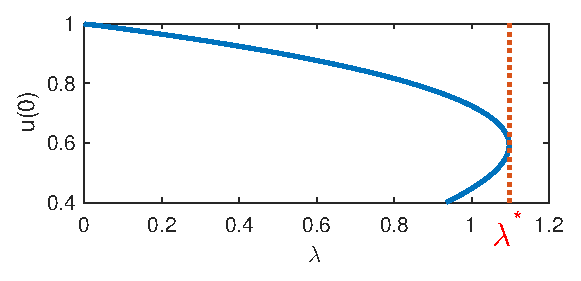
\includegraphics{strip_path}
\end{center}
(This picture is \emph{not} quantitatively accurate for your results!) 

What we really want to do is follow along the path, a technique known as \emph{continuation}. There are many ways this can be done, but this particular problem gives us a fairly easy option. The key is to observe in the figure above that $\lambda$ is a poor choice for parameterizing the path, because it fails the ``vertical line test.'' We are fortunate that in this problem, the value $u(0)$ is monotonic along the path, so it will serve as the parameter. To be specific, we solve a discretized form of~\eqref{eq:rmems} for the $n+2$ unknowns $\lambda,u_0,u_1,\ldots,u_n$. As has been our practice, the ODE is discretized at the $n-1$ interior nodes only. To this are added the \emph{three} supplemental conditions
\begin{equation}
  \label{eq:threebc}
  u'(0)=0, \qquad u(1)=1, \qquad u(0)=1-s,
\end{equation}
where $0\le s < 1$ is a value under your control. You start at $s=0$ with the trivial solution mentioned above, then gradually increase $s$ to get a sequence $s_1,s_2,\ldots$, corresponding to solutions $(\lambda_1,\bfu_1),(\lambda_2,\bfu_2)\ldots$, which are points along the path. When solving the nonlinear equations for $s=s_{k+1}$, the starting guess should be $(\lambda_k,\bfu_k)$, which is hopefully near the next point. 


\subsection*{Project assignment}
\label{sec:project-assignment}

The heart of the assignment is a function
\begin{verbatim}
[u,lambda] = mems_solve(u0,lam0,s)
\end{verbatim}
that solves the ODE with the three side conditions in~\eqref{eq:threebc}. Here \texttt{lam0} is an initial guess for $\lambda$, and the $(n+1)$-vector \texttt{u0} is an initial guess for $\bfu$. You should model this function after \texttt{bvp}, but your function does not need to solve a general problem, just the specific one at hand. Like \texttt{bvp}, your function will call \texttt{levenberg} on a subfunction named \texttt{residual}, but your version of \texttt{residual} evaluates $n+2$ quantities for values of the $n+2$ variables in a given vector $\bfz=
\begin{bmatrix}
  \lambda \\ \bfu 
\end{bmatrix}$. 
Once \verb!mems_solve! is working, you can call it within a loop to implement the steady increase of $s$. 

Your objectives are:
\begin{enumerate}
\item Find $\lambda^*$ to at least two significant digits. This means taking small enough steps along the curve as well as giving evidence that the answer has converged as a function of the discretization size $n$.
\item Find a second turning point, $\lambda^\dagger<\lambda^*$, to two digits. Past this turning point, $\lambda$ begins to increase again as a function of $s$. 
\item Make a plot like the one above for $0\le s \le 0.99$. 
\item On one graph, plot $u(r)$ against $r$ for $s=0.1,0.3,0.5,0.7,0.9,0.95$. 
\item How accurately can you find $\lambda^*$? Think about how to get the most out the discretization accuracy and how to use something more sophisticated than just taking super-small steps in $s$. Style points matter here!
\end{enumerate}

Submit a PDF report describing your results and providing any necessary supporting information. Keep it concise and to the point---for instance, don't describe multiple attempts at the last item above, just your best one. Don't forget to label your plots! Also include your \verb!mems_solve.m! and the code to reproduce the results for items~1--3 above. 

\end{document}

